\documentclass[11pt,a4paper,notitlepage]{exam}
\usepackage[utf8]{inputenc}
\usepackage{graphicx, wrapfig}

\usepackage{amsmath}
\usepackage{amsthm}
\usepackage{amssymb}
\usepackage{mathtools}
\usepackage[shortlabels]{enumitem}

\renewcommand*{\proofname}{Prova}
% bold math
\usepackage{amsbsy}

% draw pictures (and graphs)
\usepackage{tikz}

% \usepackage[usenames,dvipsnames,svgnames,table]{xcolor}

% code in latex
\definecolor{dkgreen}{rgb}{0,0.6,0}
\definecolor{gray}{rgb}{0.5,0.5,0.5}
\definecolor{mauve}{rgb}{0.58,0,0.82}
\definecolor{newink}{rgb}{0,0.1,0.25}
\usepackage{caption}
\usepackage{listings}
\lstset{frame=tb,
  language=Python,
  aboveskip=3mm,
  belowskip=3mm,
  showstringspaces=false,
  columns=flexible,
  basicstyle={\small\ttfamily},
  numbers=none,
  numberstyle=\tiny\color{gray},
  keywordstyle=\color{blue},
  commentstyle=\color{dkgreen},
  stringstyle=\color{mauve},
  breaklines=true,
  breakatwhitespace=true,
  tabsize=3
}


\usepackage{multirow}

% definition equal
\newcommand\eqdef{\mathrel{\overset{\makebox[0pt]{\mbox{\normalfont\tiny\sffamily def}}}{=}}}

% independence equal
\newcommand\eqindep{\mathrel{\overset{\makebox[0pt]{\mbox{\normalfont\tiny\sffamily indep}}}{=}}}


% independent and identically distributed equal
\newcommand\eqiid{\mathrel{\overset{\makebox[0pt]{\mbox{\normalfont\tiny\sffamily i.i.d.}}}{=}}}

% * to cdot
% \mathcode`\*="8000
% {\catcode`\*\active\gdef*{\cdot}}

% pseudo-code
\usepackage[portuguese, linesnumbered]{algorithm2e}
\newcommand\Recebe{\leftarrow}
\newcommand\Comment{\vartriangleright}
\SetKw{Devolva}{devolva}
% Example:
% \paragraph{}
% \SetAlgoNoLine
% \textsc{Título-Do-Algoritmo}($A, n$)\\
% \begin{algorithm}[H]
%   \Devolva $A$
% \end{algorithm}
%

% pair ceil
\DeclarePairedDelimiter{\ceil}{\lceil}{\rceil}

% pair ceil
\DeclarePairedDelimiter{\floor}{\lfloor}{\rfloor}

% images
\usepackage{graphicx}
\graphicspath{ {./} }
% use: \includegraphics[scale=1]{image}


\setlength{\parindent}{3em}
\setlength{\parskip}{0.5em}

\begin{document}
% \SetAlgoNoLine
\begin{center}
  %NOME E NUSP
  Nome: Rogério Marcos Fernandes Neto\hphantom{xxx} NUSP: 10284632\\
  %CURSO
  Curso: Bacharelado em Ciência da Computação\\
  %MATÉRIA
  MAC0320 - Introdução à Teoria dos Grafos
  \paragraph{}
  \textbf{LISTA 5}
\end{center}
\paragraph{E17.}Seja $G$ um grafo com $n$ vértices. Prove que se $G$ é hamiltoniano, então $\alpha(G) \leq n/2$.\medskip\\
Definição: $\alpha(G)$ denota a cardinalidade de um maior conjunto estável (ou independente)
de $G$. Um conjunto de vértices é estável (ou independente) se os seus vértices são dois a dois
não-adjacentes.

\paragraph{Solução:}
\begin{proof}
  Seja $G$ um grafo hamiltoniano de ordem $n$. Suponha, por absurdo, que $\alpha(G) > n/2$. Dessa forma, existe um conjunto independente $H \subseteq V(G)$ tal que $|H| > n/2$. Seja $H' = V(G-H)$. Como $|H| + |H'| = n$, então devemos ter $|H'| < n/2$, pois $|H| > n/2$. Assim, temos que o grafo $G-H'$ contém apenas vértices de $H$ e portanto, possui $|H|$ componentes, pois os vértices de $|H|$ não são vizinhos dois-a-dois. Dessa forma, $c(G-H') = |H| > n/2 > |H'|$, e portanto, pelo \textbf{teorema 4.1}, $G$ não pode ser hamiltoniano, contradizendo a hipótese. Portanto devemos ter $\alpha(G) \leq n/2$
\end{proof}

\paragraph{E18.}Prove que se $G$ é um grafo simples de ordem $n \geq 3$ com $|A(G)| \geq \frac{(n-1)(n-2)}{2}
  + 2$, então $G$ é hamiltoniano. Dê um exemplo de um grafo simples não hamiltoniano com n vértices e $\frac{(n-1)(n-2)}{2} + 1$ arestas. [Dica: Tentar usar uma das condições suficientes vistas.]
\paragraph{Solução:}
\begin{proof}
  Seja $G$ um grafo simples de ordem $n \geq 3$ com $|A(G)| \geq \frac{(n-1)(n-2)}{2}+2$. Como o grafo não é completo então existem vértices não adjacentes em $G$. Sejam $u$ e $v$ dois vértices não adjacentes quaisquer de $G$. Seja $X = V(G) - u - v$. Como $|X| = n-2$ então o número máximo de arestas que tem as duas pontas em $X$ é ${n-2 \choose 2} = \frac{(n-2)(n-3)}{2}$. Portanto, existem pelo menos
  $$
    \bigg(\frac{(n-1)(n-2)}{2} + 2\bigg) -  \bigg(\frac{(n-2)(n-3)}{2}\bigg) = n
  $$
  aresta com pontas em $u$ ou em $v$. Portanto $g(u) + g(v) = n$. Como $u$ e $v$ são genéricos, então, pelo \textbf{teorema 4.3 (Ore)}, $G$ é hamiltoniano.
\end{proof}
\paragraph{Exemplo: } Seja o seguinte grafo:
\begin{center}
  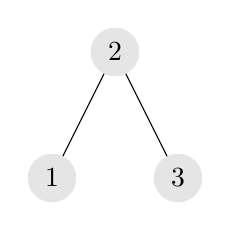
\begin{tikzpicture}
    [scale=.8,auto=left,every node/.style={circle,fill=gray!20}]
    \draw
    (0,0) node {1}
    -- (1,2) node {2}
    -- (2,0) node {3};
  \end{tikzpicture}
\end{center}
Esse grafo possui $n = 3$ vértices e possui $\frac{(n-1)(n-2)}{2} + 1 = \frac{2\cdot 1}{2} + 1 = 2$ arestas. O grafo é acíclico e portanto não pode ser hamiltoniano.

\paragraph{E19. } Seja $G$ um grafo simples de ordem $n$. Prove que se $g(u) + g(v) \geq n - 1$ para todo par de vértices não-adjacentes $u, v$ de $G$, então $G$ tem um caminho hamiltoniano.\medskip\\
\textit{OBS: Dá para fazer a prova com a técnica do cruzamento, imitando a prova vista para o Teorema de Ore; se possível, faça uma prova sem usar essa técnica, mas usando uma construção que permita usar algum resultado sobre grafos hamiltonianos.}

\paragraph{Solução: }
\begin{proof}
  Suponha que a afirmação seja falsa. Então existe um grafo sem caminho hamiltoniano maximal $G$  de ordem $n$ e para todo par de vértices $i,j \in V(G)$ não adjacentes temos que $g(i) + g(j) \geq n-1$. Ou seja, $G$ não possui um caminho hamiltoniano, mas par qualquer par de vértices não adjacentes $i,j \in V(G)$, temos que $G + ij$ possui um caminho hamiltoniano.\\
  Seja $P = (u=v_1, v_2, \dots , v_{n-1} = v)$ um caminho mais longo em $G$. Pela maximalidade de $G$ sabemos que $V(P) = n-1$. Seja $w$ o único vértice de $G$ que não está em $P$. Note que se $v_i$ é vizinho de $u$ então $v_{i-1}$ não pode ser vizinho de $w$, pois senão
  $$
    P' = (v_{n-1}, v_{n-2}, \dots, v_i,  v_1, v_2, \dots, v_{i-1}, w)
  $$
  seria um caminho hamiltoniano, contrariando a escolha de $G$. Portanto, para todo vértice adjacente a $u$ existe um vértice em $G - w$ que não é adjacente a $w$. Além disso, note que $w$ não pode ser vizinho de $v$, pois $P+vw$ seria um caminho hamiltoniano, também contrariando a escolha de $G$. Mas nesse caso,
  $$
    g(w) \leq n - 1 - g(u) - 1 \iff g(w) + g(u) \leq n - 2
  $$
  o que contraria nossa hipótese sobre o grau de vértices não adjacentes. Portanto a afirmação é verdadeira.
\end{proof}

\paragraph{E20. }Seja $G$ um grafo simples $(X, Y )$-bipartido com $|X| = |Y | = k \geq 2$. Prove que se para todo
par $u, v$ de vértices não-adjacentes tem-se que $g(u) + g(v) > k$, então $G$ é hamiltoniano.\medskip\\
$[$Sugestão: Provar por contradição, imitando a prova feita para o Teorema de Dirac, usando a técnica do cruzamento.$]$

\paragraph{Solução: }
\begin{proof}
  Suponha que a afirmação seja falsa. Então existe um grafo não hamiltoniano maximal $G$ e $(X,Y)$-bipartido com $|X| = |Y| = k \geq 2$ e para todo par de vértices $i \in X$, $j \in Y$ não adjacentes temos que $g(i) + g(j) > k$. Ou seja, $G$ não é hamiltoniano, mas para qualquer par de vértices não adjacentes $i,j \in V(G)$, temos que $G + ij$ é hamiltoniano.\\
  Se cada vértice de $X$ estivesse ligado a todos os vértices de $Y$, equivalentemente teriamos que cada vértice de $Y$ estaria de ligado a todos os vértices de $X$ e o grafo $G$ seria claramente hamiltoniano. Portanto existem dois vértices $u \in X$ e $v \in Y$ não adjacentes. Pela maximalidade de $G$ temos que o grafo $H = G + uv$ é hamiltoniano e portanto, todo circuito hamiltoniano em $H$ deve contem a aresta $uv$. Então $G$ tem um caminho hamiltoniano $P = (u=v_1, v_2, \dots, v=v_n)$.
  Note que se $v_i$ é vizinho de $u$ então $v_{i-1}$ não pode ser vizinho de $v$. Pois nesse caso teriamos que
  $$
    C = (v_1,v_i,v_{i+1},\dots, v_n,  v_{i-1}, v_{i-2}, \dots, v_1)
  $$
  seria um circuito hamiltoniano, contrariando a escolha de $G$. Portanto, para todo vértice adjacente a $u$ existe um vértice em $G - v$ que não é adjacente a $v$. Além disso, como $G$ é bipartido, então $v$ só se liga a vértices de $X$. Mas então, como $|X| = k$, temos
  $$
    g(v) \leq k - g(u) \iff g(v) + g(u) \leq k
  $$
  o que contraria nossa hipótese sobre o grau de vértices não adjacentes. Portanto a afirmação é verdadeira.
\end{proof}



\end{document}
